% Took this from CogSci but removed the header, sorry.
%
% Author: Matthew Turner
% Date: 2017-11-23

\documentclass[11pt,letterpaper]{article}

\usepackage{lineno}
\linenumbers
% \usepackage{cogsci}
\usepackage{fullpage}
\usepackage{booktabs}
\usepackage{setspace}
\doublespacing
\usepackage{pslatex}
\usepackage{hyperref}
\usepackage{url}
\usepackage{apacite}
\usepackage{amsmath}
\usepackage{subcaption}
\usepackage[utf8]{inputenc}
\usepackage{pgfplots}
\pgfplotsset{compat=newest}
\usepgfplotslibrary{groupplots}
\usepackage{wrapfig}
\usepackage{bigfoot}
\usepackage[export]{adjustbox}
\setlength\intextsep{0pt}
\usepackage{authblk}



\usepackage{graphicx}

\usepackage{gb4e}  % linguistic examples
\noautomath

\title{Polarization is sensitive to initial opinion extremity and communication noise}

\author[1]{Matthew~A.~Turner}
\author[1]{Paul~E.~Smaldino}

\affil[1]{\footnotesize Cognitive Science Program, University of California, Merced}

\date{}

\begin{document}
\maketitle

\begin{abstract}
  Opinion dynamics in general models how attributes of agents in a population
  change over time. This paper reproduces and extends the investigation of
  \citeA{Flache2011} into how cultural polarization emerges in populations
  connected on a small-world network. Their results do much to shed light
  on what might be the necessary requirements for polarization to occur.
  Importantly, opinions must be measured in a way that allows for negative
  valence of opinion, representing being ``against'' some cultural object.
  Here we add three further considerations we believe are important in 
  modeling when polarization obtains. First, we show that final polarization
  is sensitive to the initial extremity of agent opinions. Second, we quantify
  how robust polarizing dynamics are to noise. 
\end{abstract}

\section{Introduction}

\subsection{Summary of Flache and Macy (2011) model}

\section{Methods}
\label{sec:methods}

the \citeA{Flache2011}

\section{Results}

We begin by demonstrating how polarization emerges in the model under the
base parameterization of \cite{Flache2011}. Parallel 
coordinate plots for various $K$ below. At $t=0$, each agent's opinion 
features are filled with a real number between drawn from a uniform 
distribution over $[-1, 1]$. Then, 20 
ties between two randomly selected nodes are added to the network at 
iteration 2000. The system is iterated 8000 more times for 10000 total 
iterations. \citeA{Flache2011} show graphs of the state of systems for $K=2$.
As \citeA{Flache2011} showed, and we
reproduce in Figure~\ref{fig:k_finegrained}, polarization vanishes as
as the cultural complexity increases.
However, it is a well-studied fact that our everyday intuitions about 
our low-dimensional world do not always hold up in higher dimensions 
\cite{Aggarwal2001}. So, this process is illustrated for $K \geq 3$ in 
Figure~\ref{fig:parallel-coords}.   

\begin{figure}
  \centering
      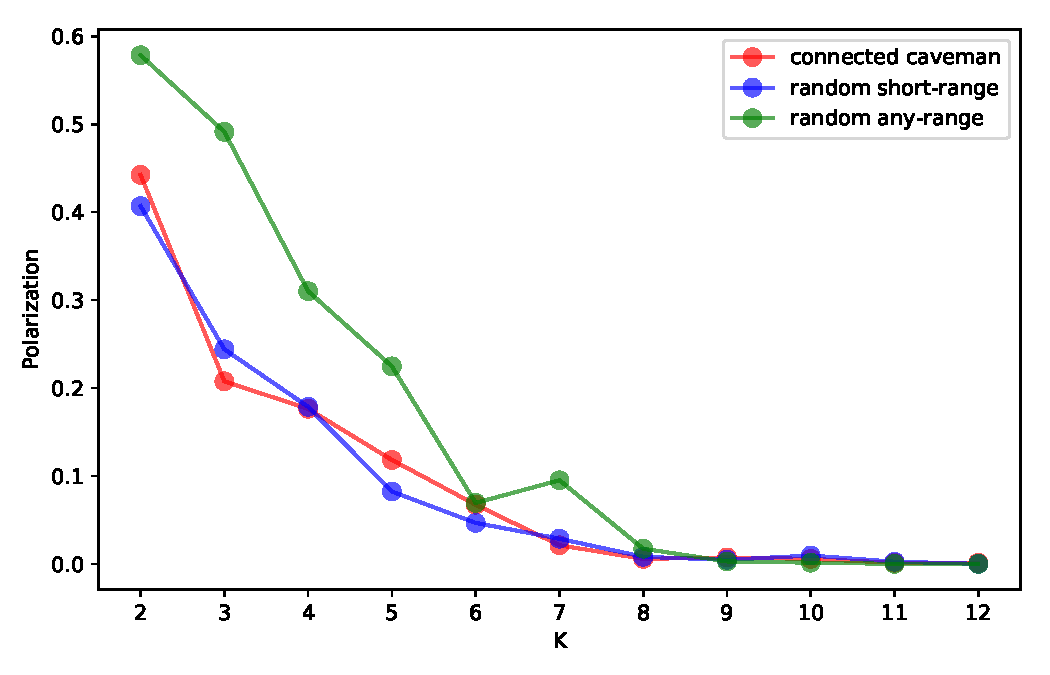
\includegraphics[width=0.75\textwidth]{Figures/finegrained_p_vs_K.pdf}
  \caption{
    Compare to FM 2011 Figure 12b. Identical, but with more intermediate
    values of cultural complexity $K$. As found by Flache and Macy, 
    average final polarization decreases with $K$. Each
    data point is the average of fifty trials. Each trial ran over 
    10k timesteps.
  }
  \label{fig:k_finegrained}
\end{figure}

\begin{figure}
  \centering
  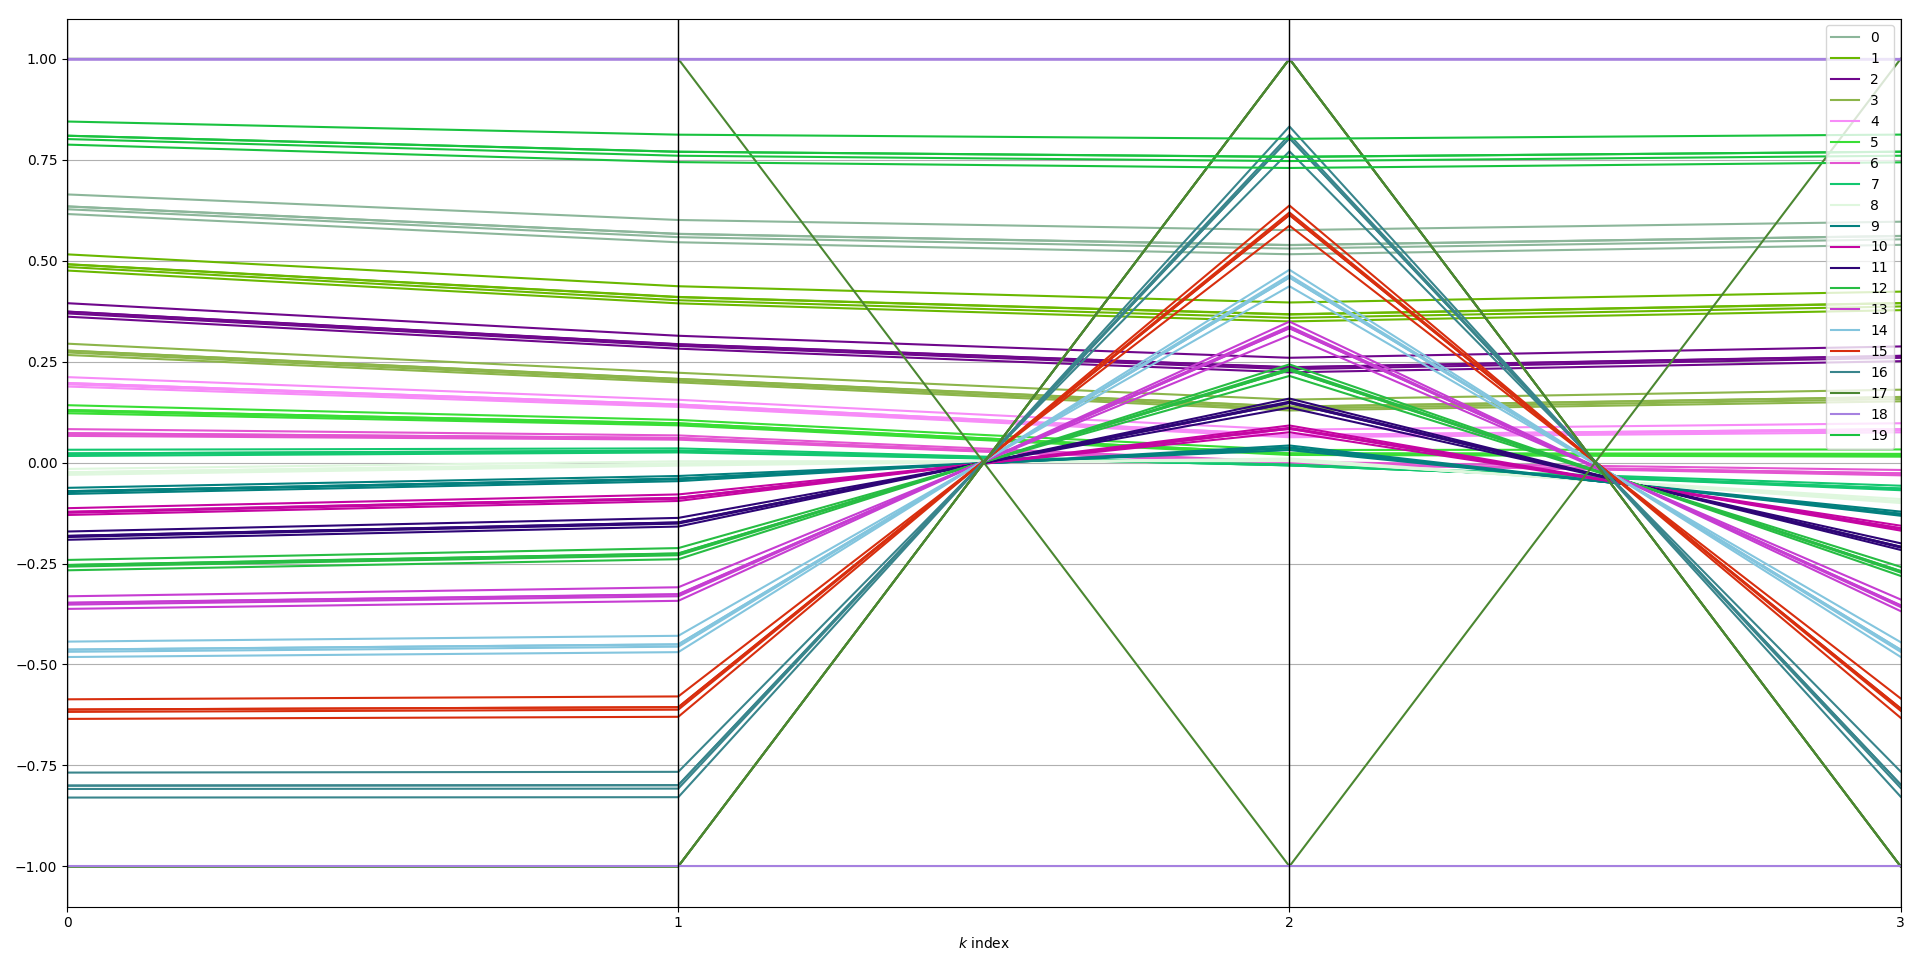
\includegraphics[width=0.75\textwidth]{parallel_coords_k=4.png}
  \caption{Tracking the evolution of opinions in model societies with varying
    cultural complexities. Each line represents a single agent. Each color
    corresponds to a different cave. 
    Each x-axis tick is one of the $K$ dimensions.
    The intersection of an agent line with each of the x-axis grid lines indicates
    the position in the $k_i$ direction. In $K=3$ dimensions, for example, 
    there would be three opinion directions, $k_1, k_2, k_3$.
    Examining the state of the system using parallel 
    coordinates allows us to see the location of the opinions in any number
    of dimensions.}
  \label{fig:parallel-coords}
\end{figure}

\subsection{Initial extremism and polarization}

\begin{figure}
  \centering
  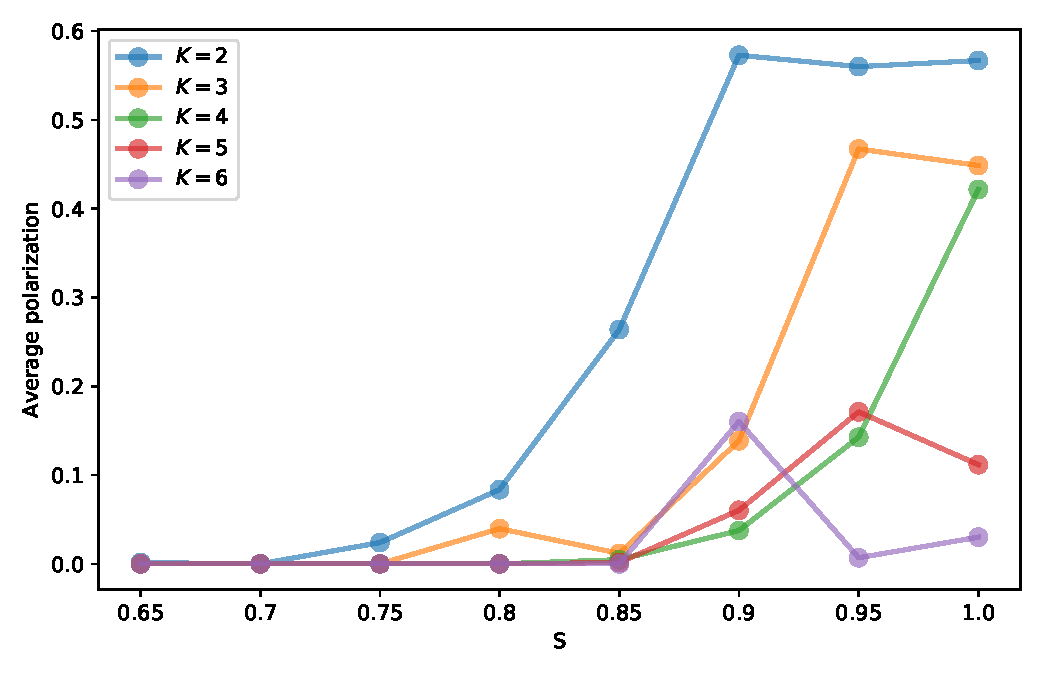
\includegraphics[width=0.75\textwidth]{Figures/P_vs_S_for_K.pdf}
  \caption{
    Average final polarization becomes non-zero then increases as
    the width of the uniform distribution of initial opinions increases.
    The width must be larger and larger as the cultural complexity $K$ 
    increases for the system to achieve non-zero final polarization. This
    condition is identical to the bottom row of each heatmap in 
    Figure \ref{fig:heatmaps}. Each
    data point is the average of fifty trials. Each trial ran over 
    10k timesteps. 
  }
  \label{fig:p_vs_s_for_k}
\end{figure}

\subsection{Communication noise and polarization}

\begin{figure}[t!]
  \centering
      \begin{subfigure}[t]{0.49\textwidth}
          \centering
          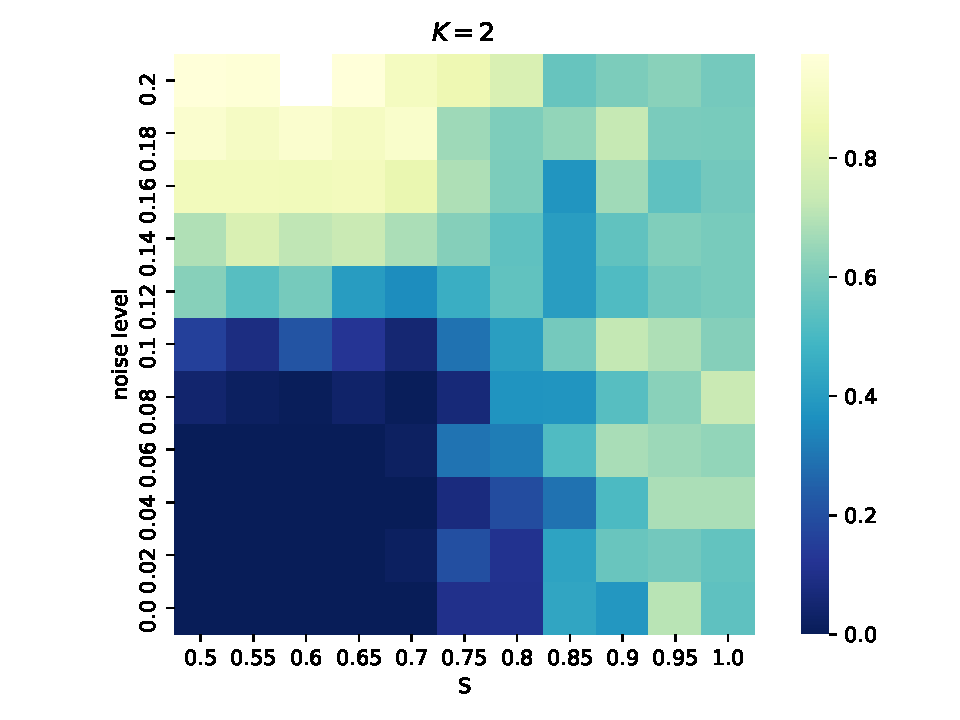
\includegraphics[width=\textwidth]{Figures/p_v_noise_k=2.pdf}
          \caption{}
      \end{subfigure}
      ~
      \begin{subfigure}[t]{0.49\textwidth}
          \centering
          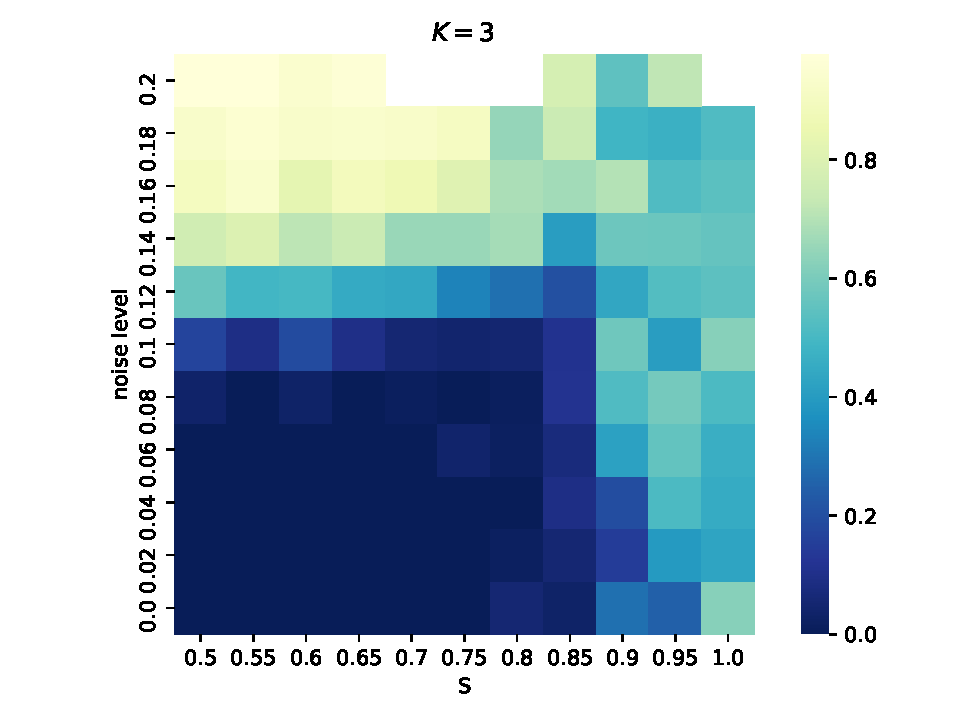
\includegraphics[width=\textwidth]{Figures/p_v_noise_k=3.pdf}
          \caption{}
      \end{subfigure} \\
      \begin{subfigure}[t]{0.49\textwidth}
          \centering
          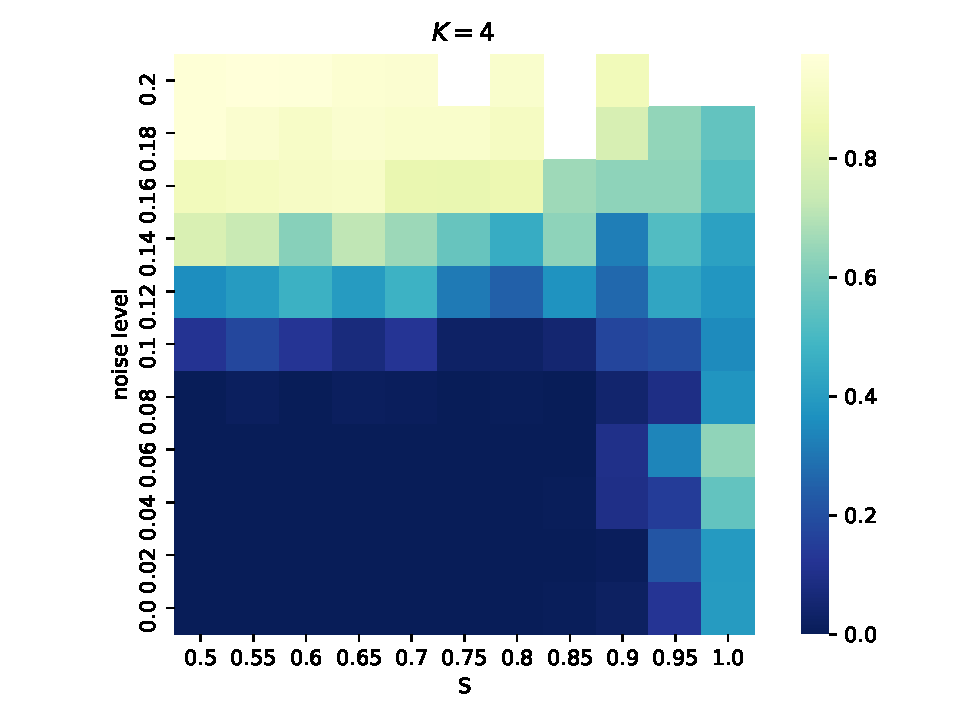
\includegraphics[width=\textwidth]{Figures/p_v_noise_k=4.pdf}
          \caption{}
      \end{subfigure}
      ~
      \begin{subfigure}[t]{0.49\textwidth}
          \centering
          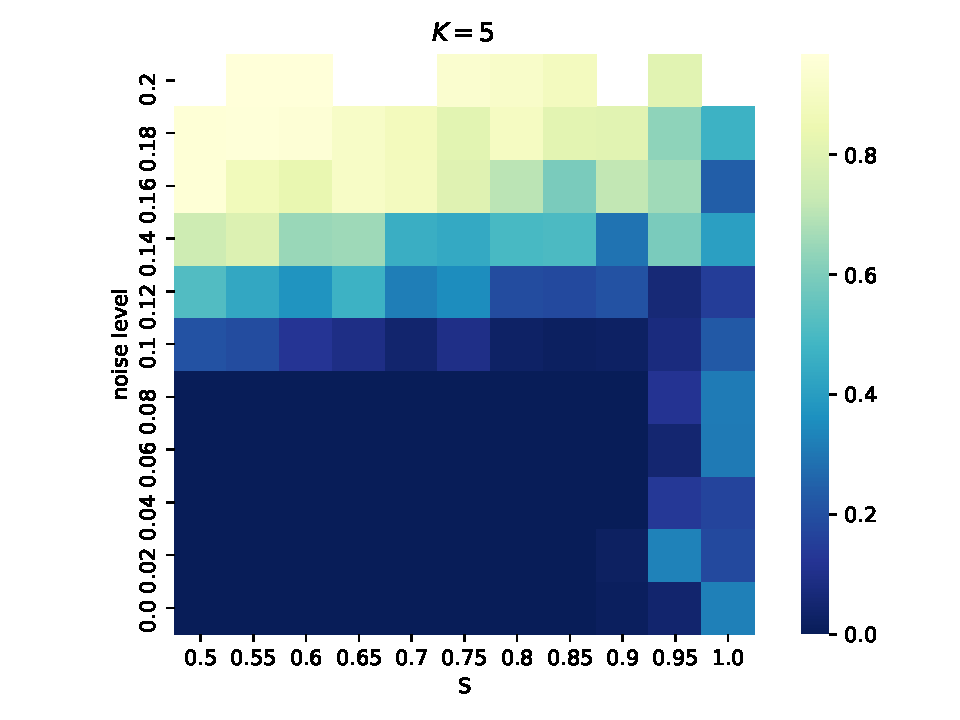
\includegraphics[width=\textwidth]{Figures/p_v_noise_k=5.pdf}
          \caption{}
      \end{subfigure} \\
  \caption{Final average polarization varies with both the width of the
    uniform distribution of initial opinion magnitudes and the noise level in
    the opinion updates. Noisy opinion updates can perturb the system away from
    situations where homogeneity of opinion would otherwise obtain. $K=2,3,4,5$
    are shown. The value in each square of the heatmap is the average of
    fifty trials. Each trial ran over 10k timesteps.
  }
  \label{fig:heatmaps}
\end{figure}




\bibliographystyle{apacite}

\setlength{\bibleftmargin}{.125in}
\setlength{\bibindent}{-\bibleftmargin}

\bibliography{/Users/mt/workspace/papers/library.bib}

\end{document}
